\documentclass[12pt, twoside]{article}
\input{/Users/chris/github/course-files/docs/ib/preamble}
\setlength{\parskip}{0.3\baselineskip}

\fancyhead[LE]{\thepage}
\fancyhead[RO]{Markscheme}
\fancyhead[LO]{La Scuola d'Italia / Dr.\ Huson / IB Math 12 HL \\* 29 September 2026}

\begin{document}
\subsubsection*{12.5 Classwork: Roots of Complex Numbers --- Markscheme}

\emph{No calculator. Marks are not printed on the student sheet; they are
recorded here. Total: 26 marks.}

\begin{enumerate}[itemsep=0.3cm]

%--- Problem 1: Square roots of 5 - 12i; complex quadratic; not a conjugate pair [6 marks] ---
\item[1.] [Maximum mark: 6]

\textbf{(a)} $(a + bi)^{2} = a^{2} - b^{2} + 2abi = 5 - 12i$, so
$a^{2} - b^{2} = 5$ \ and \ $2ab = -12$ \hfill \textbf{M1}

Substituting $b = -\dfrac{6}{a}$: \ $a^{2} - \dfrac{36}{a^{2}} = 5$, \
$a^{4} - 5a^{2} - 36 = 0$, \ $(a^{2} - 9)(a^{2} + 4) = 0$

$a^{2} = 9$ (since $a$ is real), so $a = \pm 3$, $b = \mp 2$
\hfill \textbf{A1}

The square roots are $3 - 2i$ and $-3 + 2i$. \hfill \textbf{A1}

\emph{M1 for expanding and equating both real and imaginary parts. Accept the
modulus shortcut $a^{2} + b^{2} = |5 - 12i| = 13$, which with
$a^{2} - b^{2} = 5$ gives $a^{2} = 9$, $b^{2} = 4$ directly. A1 for
$a = \pm 3$ with $b = \mp 2$; A1 for both roots paired correctly. Pairing the
signs wrongly ($3 + 2i$) earns the M1 only --- $2ab = -12$ forces opposite
signs. Accept $\pm(3 - 2i)$.}

\textbf{(b)} $z = \dfrac{2 \pm \sqrt{4 - 4(-4 + 12i)}}{2}
= \dfrac{2 \pm \sqrt{4(5 - 12i)}}{2} = 1 \pm (3 - 2i)$ \hfill \textbf{M1}

$z = 4 - 2i$ \ or \ $z = -2 + 2i$ \hfill \textbf{A1}

\emph{M1 for reducing the equation to a square root of $5 - 12i$, by the
quadratic formula or by completing the square, $(z - 1)^{2} = 5 - 12i$. A1 for
both solutions. The ``hence'' means the root from (a) must be used; a
candidate who restarts with $z = x + yi$ and solves correctly earns full marks
with the feedback note that (a) had already done the work. FT: award the A1 for
$1 \pm$ the candidate's own square root from (a).}

\textbf{(c)} The coefficient $-4 + 12i$ is not real. Non-real roots come in
conjugate pairs only when every coefficient is real, so the theorem does not
apply here. \hfill \textbf{R1}

\emph{R1 requires the reason to name the non-real coefficient. ``Because
$4 - 2i$ and $-2 + 2i$ are not conjugates'' only restates the question and
earns nothing.}

\newpage

%--- Problem 2: Fourth roots of -8 + 8sqrt3 i [7 marks] ---
\item[2.] [Maximum mark: 7]

\textbf{(a)} $|w| = \sqrt{(-8)^{2} + (8\sqrt{3})^{2}} = \sqrt{256} = 16$
\hfill \textbf{A1}

$w$ is in the second quadrant with $\tan\alpha = \sqrt{3}$, so
$\arg w = \pi - \dfrac{\pi}{3} = \dfrac{2\pi}{3}$ \hfill \textbf{A1}

$w = 16e^{2\pi i/3}$

\emph{The marks are independent. $\arg w = -\dfrac{\pi}{3}$ (from
$\arctan(-\sqrt{3})$ with no quadrant check) loses the second A1. Accept
$16\operatorname{cis}\dfrac{2\pi}{3}$.}

\textbf{(b)} $z^{4} = 16e^{i(2\pi/3 + 2k\pi)}$, so
$z = 2e^{i(\pi/6 + k\pi/2)}$ \hfill \textbf{M1}

$k = 0, 1$: \ $z = 2e^{i\pi/6}, \ 2e^{2\pi i/3}$ \hfill \textbf{A1}

$k = -1, -2$: \ $z = 2e^{-i\pi/3}, \ 2e^{-5\pi i/6}$ \hfill \textbf{A1}

\emph{M1 for the modulus $\sqrt[4]{16} = 2$ with the argument
$\dfrac{2\pi/3 + 2k\pi}{4}$, or for one root followed by rotations of
$\dfrac{\pi}{2}$. A1 for any two correct roots; A1 for all four with every
argument in $-\pi < \theta \leq \pi$. $2e^{7\pi i/6}$ and $2e^{5\pi i/3}$ are
outside the range and lose the final A1 unless converted. FT: award the
marks from the candidate's own $r$ and $\theta$ in (a).}

\textbf{(c)} $2e^{i\pi/6} = 2\left(\dfrac{\sqrt{3}}{2} + \dfrac{1}{2}i\right)
= \sqrt{3} + i$ \hfill \textbf{A1}

\emph{FT: award A1 for the candidate's own first-quadrant root from (b)
correctly converted.}

\textbf{(d)} $-8 - 8\sqrt{3}\,i = \overline{w}$, so the solutions are the
conjugates of those in (b):

$z = 2e^{-i\pi/6}, \ 2e^{-2\pi i/3}, \ 2e^{i\pi/3}, \ 2e^{5\pi i/6}$
\hfill \textbf{A1}

\emph{A1 for all four. Since $\overline{z}^{\,4} = \overline{z^{4}}$, each
conjugate root solves the conjugate equation. Accept solving
$z^{4} = 16e^{-2\pi i/3}$ from the start. FT: award A1 for the conjugates of the
candidate's own roots from (b).}

\newpage

%--- Problem 3: Cube roots of unity; (z - 1)^3 = 8; real factorization [7 marks] ---
\item[3.] [Maximum mark: 7]

\textbf{(a)} $z^{3} = 1 = e^{2k\pi i}$, so $z = e^{2k\pi i/3}$,
$k = 0, 1, -1$ \hfill \textbf{M1}

$z = 1, \quad -\dfrac{1}{2} + \dfrac{\sqrt{3}}{2}i, \quad
-\dfrac{1}{2} - \dfrac{\sqrt{3}}{2}i$ \hfill \textbf{A1}

\emph{Accept the factor route: $z^{3} - 1 = (z - 1)(z^{2} + z + 1) = 0$, then
the quadratic formula on $z^{2} + z + 1 = 0$. A1 for all three in Cartesian
form; answers left as $e^{\pm 2\pi i/3}$ earn the M1 only.}

\textbf{(b)} $\left(\dfrac{z - 1}{2}\right)^{3} = 1$, so
$z - 1 = 2, \ \ 2\left(-\dfrac{1}{2} \pm \dfrac{\sqrt{3}}{2}i\right)
= -1 \pm \sqrt{3}\,i$ \hfill \textbf{M1}

$z = 3, \quad \sqrt{3}\,i, \quad -\sqrt{3}\,i$ \hfill \textbf{A1}

\emph{M1 for $z - 1 = 2\omega$ with $\omega$ each cube root of unity from (a).
A1 for all three solutions. Finding only $z = 3$ earns nothing. FT: award
the marks for $1 + 2\omega$ with the candidate's own roots from (a).}

\textbf{(c)} $(z - 1)^{3} = z^{3} - 3z^{2} + 3z - 1$ \hfill \textbf{M1}

so $(z - 1)^{3} = 8 \iff z^{3} - 3z^{2} + 3z - 9 = 0$ \hfill \textbf{AG}

The roots $\pm\sqrt{3}\,i$ are a conjugate pair:
$(z - \sqrt{3}\,i)(z + \sqrt{3}\,i) = z^{2} + 3$ \hfill \textbf{M1}

$z^{3} - 3z^{2} + 3z - 9 = (z - 3)(z^{2} + 3)$ \hfill \textbf{A1}

\emph{First M1 for the binomial expansion of $(z - 1)^{3}$ with coefficients
$1, 3, 3, 1$ and alternating signs. Second M1 for any valid route to the
factors: pairing the conjugate roots from (b), grouping
$z^{2}(z - 3) + 3(z - 3)$, or dividing by $(z - 3)$. A1 for
$(z - 3)(z^{2} + 3)$. A factorization with non-real coefficients, such as
$(z - 3)(z - \sqrt{3}\,i)(z + \sqrt{3}\,i)$, earns the second M1 only ---
the question asks for a real quadratic factor.}

\newpage

%--- Problem 4: One cube root given; find w, the other roots, triangle area [6 marks] ---
\item[4.] [Maximum mark: 6]

\textbf{(a)} $1 + \sqrt{3}\,i = 2e^{i\pi/3}$ \hfill \textbf{M1}

$w = \left(2e^{i\pi/3}\right)^{3} = 8e^{i\pi} = -8$ \hfill \textbf{A1}

\emph{M1 for the exponential or polar form of $1 + \sqrt{3}\,i$ (modulus $2$,
argument $\dfrac{\pi}{3}$). A1 for $w = -8$. A correct binomial expansion of
$(1 + \sqrt{3}\,i)^{3}$ reaching $-8$ also earns full marks, with the feedback
note that the question asked for de Moivre.}

\textbf{(b)} The cube roots of $w$ are $2e^{i\pi/3}$ rotated by
$\pm\dfrac{2\pi}{3}$: \hfill \textbf{M1}

$2e^{i\pi} = -2$ \ and \ $2e^{-i\pi/3} = 1 - \sqrt{3}\,i$ \hfill \textbf{A1}

\emph{M1 for any valid method: rotation by $\dfrac{2\pi}{3}$, solving
$z^{3} = 8e^{i(\pi + 2k\pi)}$, or the conjugate root theorem ($z^{3} + 8 = 0$
has real coefficients, so $1 - \sqrt{3}\,i$ is a root) with the third root
from the sum of roots $= 0$ or from $z = -2$ by inspection. A1 for both roots
in Cartesian form. FT: award the marks for the cube roots of the candidate's
own $w$.}

\textbf{(c)}

\begin{center}
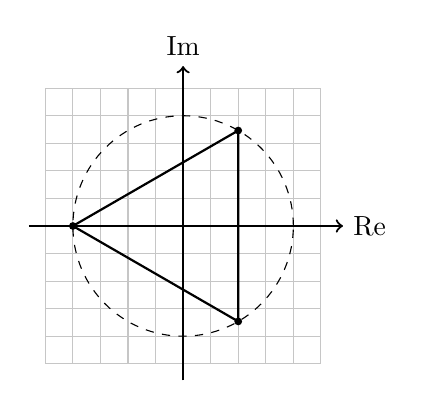
\begin{tikzpicture}[scale=0.7]
  \draw [thin, color=gray!45, step=0.5cm] (-2.5,-2.5) grid (2.5,2.5);
  \draw [thick, ->] (-2.8,0) -- (2.9,0) node [right] {$\mathrm{Re}$};
  \draw [thick, ->] (0,-2.8) -- (0,2.9) node [above] {$\mathrm{Im}$};
  \draw [thick] (1,1.732) -- (-2,0) -- (1,-1.732) -- cycle;
  \draw [dashed] (0,0) circle (2);
  \foreach \p in {(1,1.732), (-2,0), (1,-1.732)} \fill \p circle (2pt);
\end{tikzpicture}
\end{center}

The side from $1 + \sqrt{3}\,i$ to $1 - \sqrt{3}\,i$ has length $2\sqrt{3}$,
and the height from $-2$ to the line $\mathrm{Re}(z) = 1$ is $3$.
\hfill \textbf{M1}

$\text{Area} = \dfrac{1}{2} \times 2\sqrt{3} \times 3 = 3\sqrt{3}$
\hfill \textbf{A1}

\emph{M1 for any valid area method: base and height as above, the equilateral
formula $\dfrac{\sqrt{3}}{4}s^{2}$ with $s = 2\sqrt{3}$, or three triangles from
the origin, $3 \times \dfrac{1}{2}(2)(2)\sin\dfrac{2\pi}{3}$. A1 for
$3\sqrt{3}$. A decimal answer ($5.20$) loses the A1: the question asks for the
exact area. FT: award the marks from the candidate's own roots in (b).}

\end{enumerate}
\end{document}
